\section{LIME}

LIME \cite{ribeiro2016should} is a black box interpretability method. Like all black box methods, LIME randomly changes features in the input data to detect which feature is relevant for the classification. The output of LIME is a list of features which the algorithm detected as to be relevant for the classification, sorted by importance.

In the case of image classification, LIME does not modify single pixels, because this would generate too many different versions of the input.
Instead, LIME generates superpixels.

\begin{figure}[H]
\centering
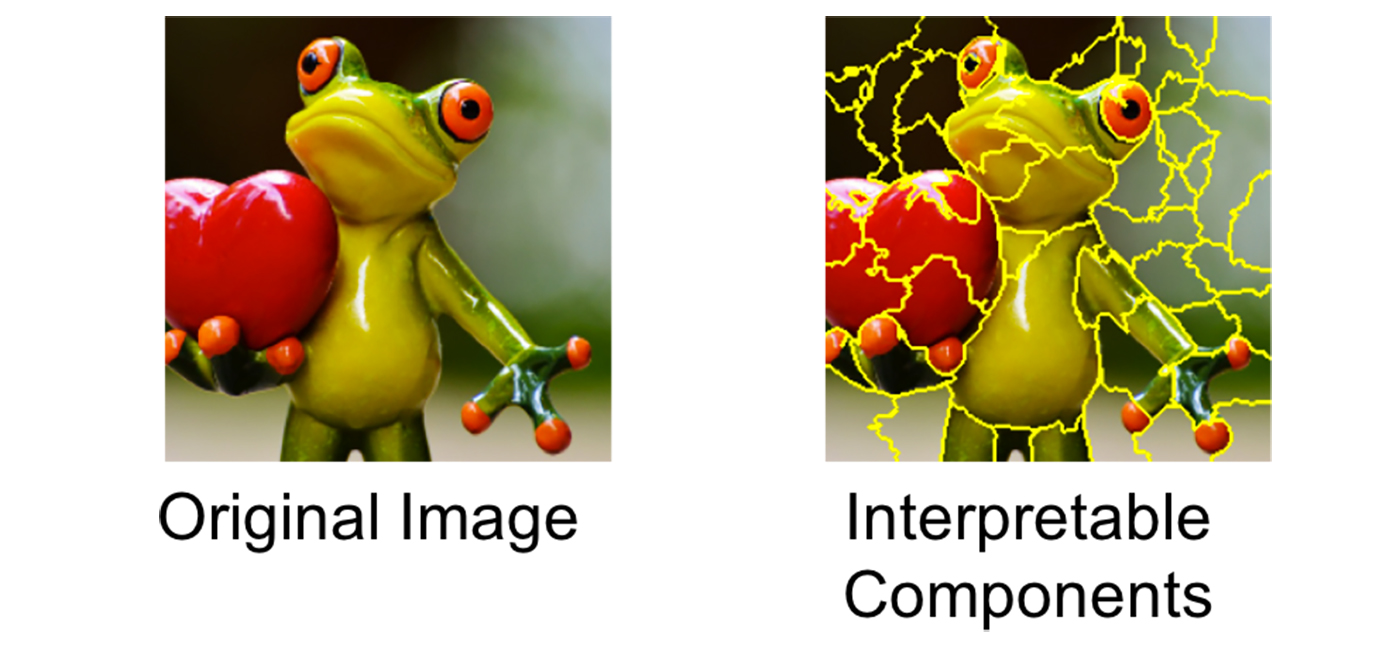
\includegraphics[width=12cm]{chapters/02_methods/images/lime.jpg}
\caption{Superpixels generated for an input image. Superpixels are the features LIME analyzes to detect if they are relevant for the classification.\cite{limeoreilly}}
\label{lime_superpixel}
\end{figure}

Superpixels are continuous regions on an image with a similar color. In the Python reference implementation, LIME uses the Quick Shift \cite{vedaldi2008quick} clustering algorithm to generate these superpixels. Figure \ref{lime_superpixel} shows superpixels overlaid on an example image.

\begin{figure}[H]
\centering
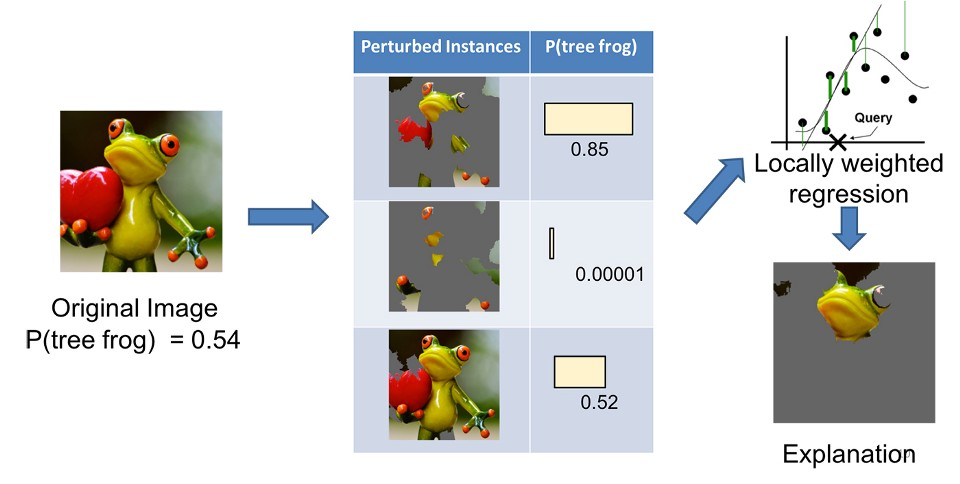
\includegraphics[width=14cm]{chapters/02_methods/images/lime2.jpg}
\caption{Left: Original image with detected class and probability. Middle: Perturbed images by randomly turned off superpixels and their probability for the specific class.
Right: Locally weighted regression to generate a preferably continuous region to explain the class.\cite{limeoreilly}}
\label{lime_perturbed}
\end{figure}

In the next step, LIME generates input images by turning off multiple randomly selected superpixels. Turning off in this case means setting the color inside the superpixel to gray. The center image of Figure \ref{lime_perturbed} shows some examples of deactivated superpixels. The generated input images are then run trough the neural network and the changed probabilities of the relevant class(es) are recorded. As a last step, LIME does a locally weighted (i.e. adjacent superpixels are weighted higher) regression of the probabilities to generate a preferably continuous cluster of superpixels explaining a specific class (right image in Figure \ref{lime_perturbed}).

Figure \ref{lime_dog} shows some example explanation for a complex input image.

\begin{figure}[H]
    \centering
    \begin{subfigure}[t]{.23\textwidth}
        \centering
        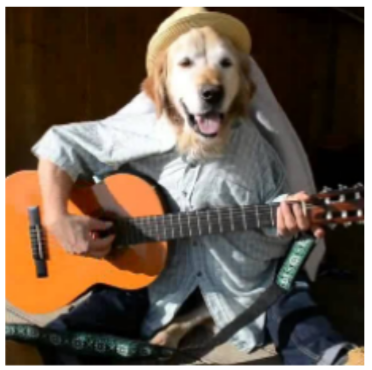
\includegraphics[width=\linewidth]{chapters/02_methods/images/lime_dog_1.png}
        \caption{Original image}
    \end{subfigure}\hfill%
    \begin{subfigure}[t]{.23\textwidth}
        \centering
        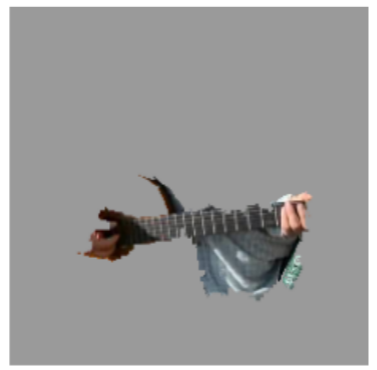
\includegraphics[width=\linewidth]{chapters/02_methods/images/lime_dog_2.png}
        \caption{Explain class Electric guitar}
    \end{subfigure}\hfill%
    \begin{subfigure}[t]{.23\textwidth}
        \centering
        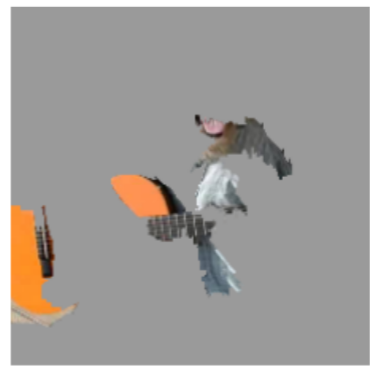
\includegraphics[width=\linewidth]{chapters/02_methods/images/lime_dog_3.png}
        \caption{Explain class Acoustic guitar}
    \end{subfigure}\hfill%
    \begin{subfigure}[t]{.23\textwidth}
        \centering
        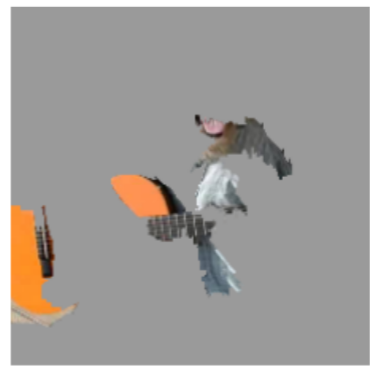
\includegraphics[width=\linewidth]{chapters/02_methods/images/lime_dog_3.png}
        \caption{Explain class Labrador}
    \end{subfigure}
    \caption{Explaining the top 3 classes on an example image with LIME. b) is class "Electric guitar" with p=0.32, c) is "Acoustic guitar" with p=0.24, d) is "Labrador" with p=0.21}
    \label{lime_dog}
\end{figure}
